\chapter{Examples}

This chapter demonstrates the usage of our solution by four examples, which are inspired by the use cases mentioned earlier.
We describe example structure, show important blocks of code, which has to be added to project.
At the end, we make snapshots of the websites.
\par

\section{WebGame}

The example aims at the third use case.
It contains a game where we have a rocket, which has to destroy falling asteroids with bullets, as we can see in Figure \ref{img28:game}.
We can also see current \ac{FPS} in the left corner of the screenshot.
The rocket can be control by buttons in the bottom, or we can use a keyboard, where arrows determine the rocket movement and \texttt{F} key fires a bullet.
We will discuss the rendering time in the benchmark section.
\par
\begin{figure}\centering
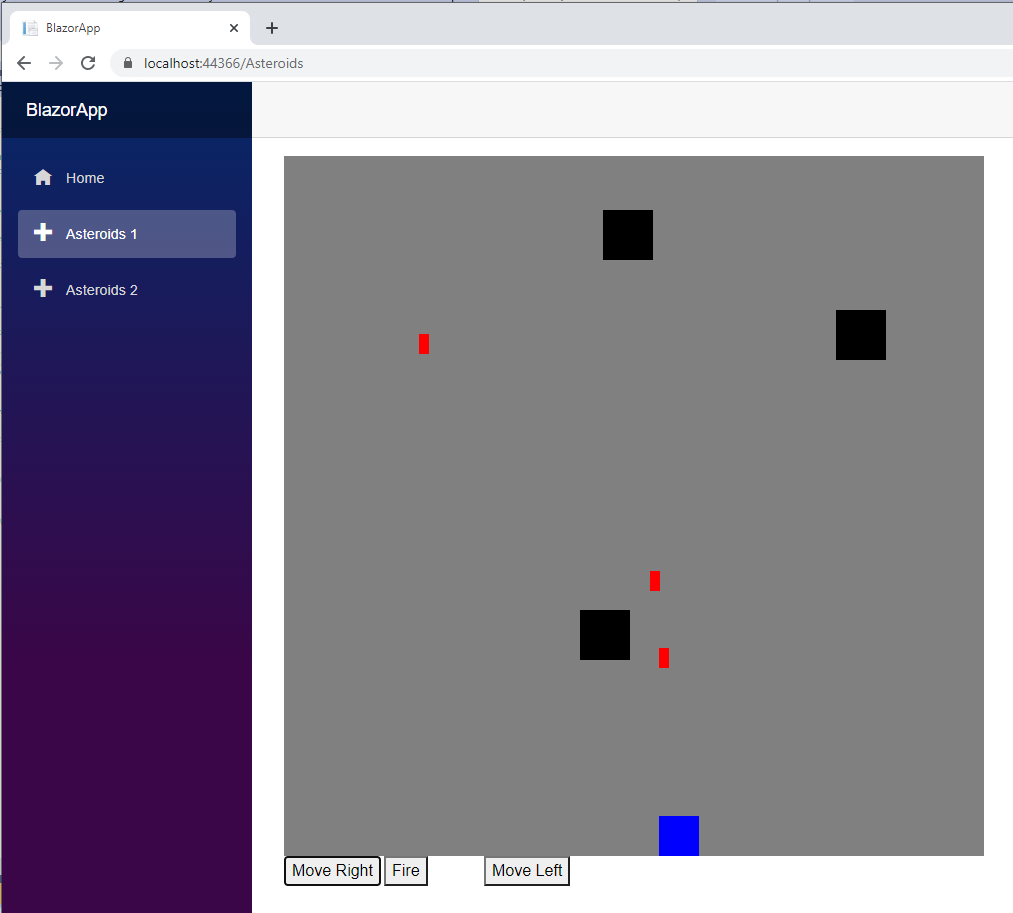
\includegraphics[scale=0.5]{./img/Asteroids}
\caption{The game.}
\label{img28:game}
\end{figure} 
\par
The example is implemented as .NET solution consisting of three projects. 
\texttt{BlazorApp.Client} and \texttt{BlazorApp.Server} are pregenerated projects by the Blazor App template.
The game is implemented in the Peachpie \texttt{PHPScripts} project.
These projects reference the \texttt{Peachpie.Blazor} library as a NuGet package containing our solution. 
We describe steps, which was necessary for making the game working.
\par
The game implementation is contained in three PHP scripts and a CSS file containing game styles.
The \textit{settings.php} script contains default values of FPS, an asteroids frequency, and additional settings.
The \textit{asteroids.php} script contains definitions of game entities like the rocket or an asteroid.
These entities utilizes \texttt{Peachpie.Blazor} library, which provides helper classes representing HTML elements.
At the bottom of the script is \texttt{Application} class connecting all parts together.
The class uses HTML elements events for interacting with the user due to the \texttt{PhpTreeBuilder} class providing an API targeting PHP usage.
The last script is \textit{main.php}, which contains \texttt{AsteroidsComponent} class.
This class is routable by \texttt{/Asteroids} URL and initializes the game.
It uses \texttt{Timer} provided by \texttt{Peachpie.Blazor}, which enables to handles tick events, which update the game and the screen.
Because \texttt{Application} class inherits the helper class \texttt{Tag}, \texttt{AscteroidsComponent} does not bother with game rendering and uses \texttt{BlazorWritable} interface for transparent initiating the rendering.
\par
\texttt{BlazorApp.Client} references the game and uses the default \texttt{Router} component to navigate \texttt{AsteroidsComonent}.
\texttt{index.html} contains links to the game styles and a supporting Javascript defined in the \texttt{Peachpie.Blazor} library.
We can see two examples of \texttt{AsteroidsComponent} usage in Figure \ref{img28:game}.
\textit{Asteroids 1} utilizes the router for navigating it.
\textit{Asteroids 2} utilizes a Razor page, which contains additional content with the game.
\par
\texttt{BlazorApp.Server} provides the Web Static Assets to a client by inserting additional middlewares, which handles their requests.
This insertion can be seen in the \textit{Startup.cs} file and in Figure \ref{img21:server}.
The website is run by launching the server.
\par
\begin{figure}
\begin{lstlisting}
var fileProvider = new ManifestEmbeddedFileProvider(
	typeof(PhpBlazor.BlazorContext).Assembly);
app.UseStaticFiles(new StaticFileOptions() {
	 FileProvider = fileProvider });

app.UseStaticFiles(new StaticFileOptions
{
	FileProvider = new PhysicalFileProvider(
		Path to static resources, "PHPScripts\\wwwroot")),
	RequestPath = "/Asteroids"
});
\end{lstlisting}
\caption{A part of the \texttt{Configure} method contained in the \texttt{StartUp} class, which is defined in \textit{Startup.cs}}
\label{img21:server}
\end{figure}

\section{Web}

Web example is inspired by the first use case, which moves the website on a client side.
The website contains a simple layout consisting of references to the website parts.
We can see the default page in Figure \ref{img28:website}.
The website contains images, which are downloaded from the server when they are required.
\par
\begin{figure}[!b]\centering
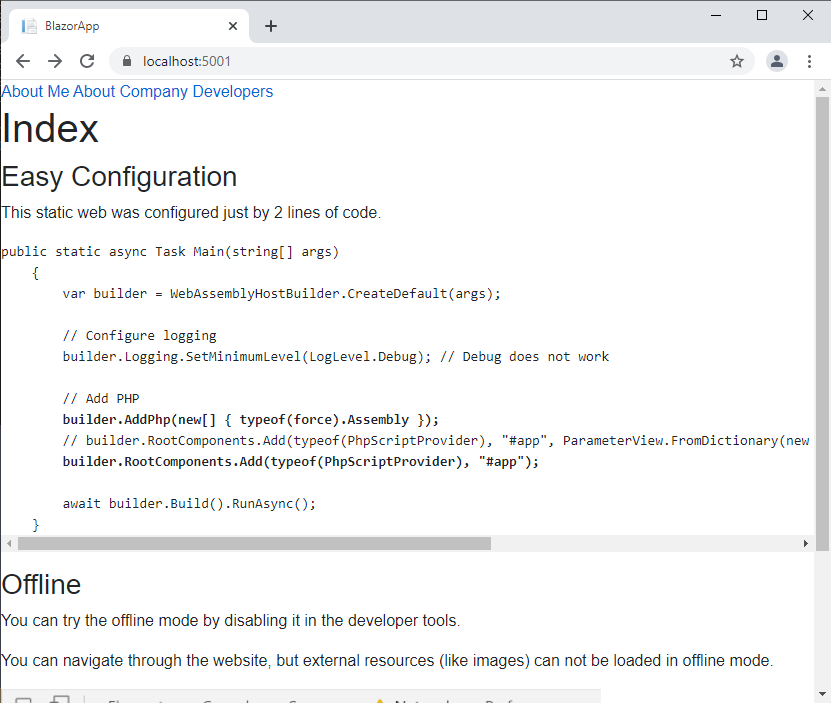
\includegraphics[scale=0.5]{./img/Web}
\caption{The default page.}
\label{img28:website}
\end{figure} 
\par
The whole application is implemented as .NET solution consisting of three projects.
\texttt{BlazorApp.Client} represents the client application containing \texttt{Program.cs}, which sets \texttt{WebAssemblyBuilder} with a root component, \texttt{PhpScriptProvider}, as we can see in Figure \ref{img20:program}.
\texttt{Blazor.Server} has the same role as in the previous example.
\par
\begin{figure}
\begin{lstlisting}
public static async Task Main(string[] args)
{
	var builder = WebAssemblyHostBuilder.CreateDefault(args);

	// Configure logging
	builder.Logging.SetMinimumLevel(LogLevel.Debug);

	// Add PHP
	builder.AddPhp(new[] { typeof(force).Assembly });
	builder.RootComponents.Add(typeof(PhpScriptProvider), "#app");
            
	await builder.Build().RunAsync();
}
\end{lstlisting}
\caption{The Main method in Program.cs}
\label{img20:program}
\end{figure}
\par
The project references \texttt{Peachpie.Blazor} library and the Peachpie project, \texttt{PHPScripts}, containing PHP scripts representing the website.
The provider has default settings, which are the \texttt{Router} type and the \texttt{OnNavigationChanged} mode of \texttt{BlazorContext}.
Furthermore, we have to link the Javascript script from \texttt{Peachpie.Blazor} library to \textit{index.html} in order to use it during the runtime.
\par
The \texttt{PHPScripts} project contains the programmer's defined PHP scripts forming the web of some software company.
We can see the project content in Figure \ref{img22:web}.
The project uses Peachpie \ac{SDK} for compiling the scripts.
The website has a simple layout defined in \textit{defaultLayout.php} referencing pages about the founder, the company, and the community.
The \textit{me.php} page contains an image, \textit{logo.png}, which is loaded by a common tag, \texttt{<img alt="Logo" src="Web/images/logo.png"/>}.
We can see the \textit{force.php} script containing empty \texttt{force} class, which is used in \texttt{BlazorApp.Client} to force loading of this assembly to a client.
\par
\begin{figure}\centering
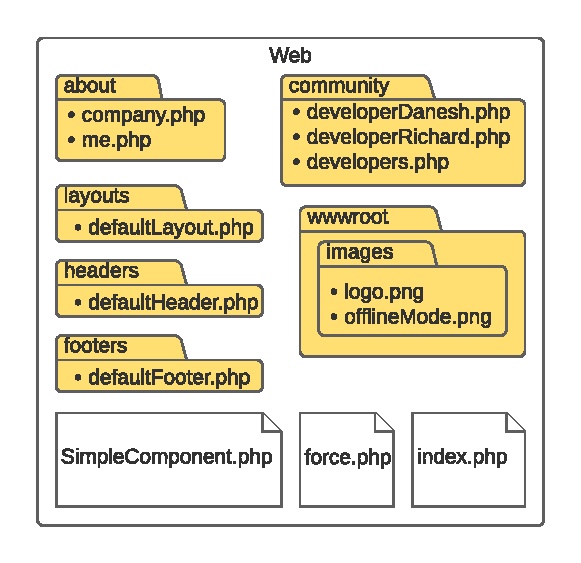
\includegraphics[scale=0.9]{./img/WebStructure}
\caption{The Web solution structure.}
\label{img22:web}
\end{figure} 
\par
An interesting page is \textit{developers.php}, which displays information about developers working in the company.
We can see the script in Figure \ref{img25:developer}
It uses script inclusion to add the head section.
Then, there is a Javascript call, which uses our predefined API, which causes showing the alert with the message when the page loads.
The whole page uses HTML interleaving.
We can see using \texttt{\$\_GET} superglobal in the script, where we decide to show its content based on the URL query.
When we have the \textit{OnNavigationChanged} mode for the context, and we refresh the page after navigation to a developer, then we can see the anchors to developers.
It is caused by creating a new context between navigation, so the variables are disposed.
With the second mode of context,\texttt{Persistant}, we still have the info page of the firstly navigated developer because the variables in the context remain.
This page is transparently rendered by our \texttt{PhpScriptProvider}, which evaluates the whole script and adds the output as a markup text to the builder.
\par
\begin{figure}
\begin{lstlisting}
<?php
    require("/headers/defaultHeader.php");
    CallJsVoid("window.alert", "Hello from PHP script.");
?>
<?php
if (isset($_GET["developer"])) { 
    $name = $_GET["developer"];
    require("/community/developer$name.php");
} else {
?>
...
<p>Get more info about 
<a href="/community/developers.php?developer=Richard">Richard</a>.
</p>
...
<?php } ?>
<?php
    require("/footers/defaultFooter.php");
?>
\end{lstlisting}
\caption{developers.php}
\label{img25:developer}
\end{figure}

\section{OneScript}

In this example, we aim at the second use case.
The website contains several pages with demonstrates inserting page fragments written in PHP to the Blazor website.
When we navigate the page, we can see a button, which utilizes interoperability between PHP and Javascript provided by our solution.
When we click on it, the javascript code calls PHP code, which writes a message to a browser console.
Next examples referred as \textit{Example 1}, \textit{Example 2}, \textit{Example 3} show working with forms.
The first example uses a simple form with the \texttt{GET} method.
When we submit the form, we are navigated to a page written in PHP, displaying the content of superglobals.
The same process is done with the \texttt{POST} method.
We can also try to load a file to the form in the last example.
After the submit, the page displays its file contect encoded into \textit{base64} encoding.
\textit{Example 4} uses previously mentioned features to enable displaying user defines graphs.
We can upload a file containing the graph, or the application will generate it.
Then the graph is displayed, and we can download the points defining it as we can see in Figure \ref{img27:graph}.
\par
\begin{figure}\centering
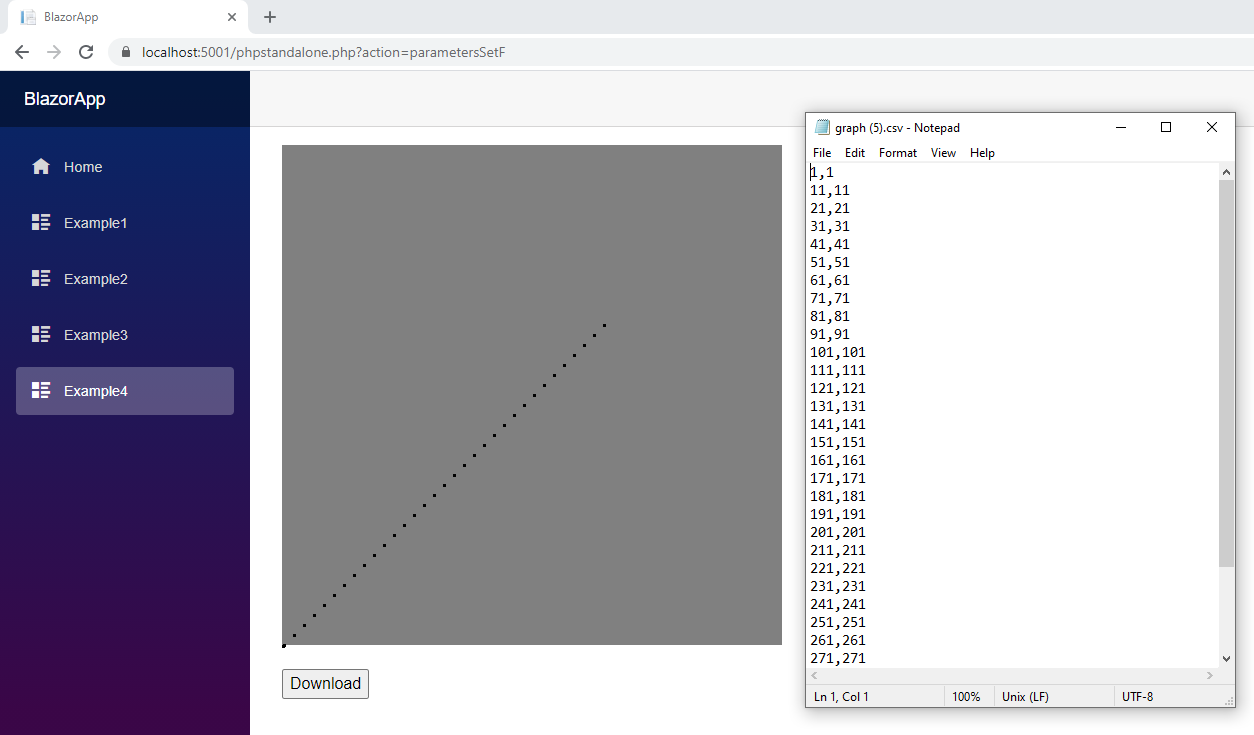
\includegraphics[scale=0.4]{./img/graph}
\caption{Application for visualising a graph.}
\label{img27:graph}
\end{figure} 
\par
The .NET solution consists of three projects.
\texttt{BlazorApp.Server} is the same as previois ones.
\texttt{BlazorApp.Client} contains common Razor pages, and has default \texttt{Router} as a root component.
We create several scripts in the Peachpie\texttt{PHPScripts} project to enrich the website with all content except the layout, which we presented.
The website contains three Razor pages: \textit{Index.razor}, \textit{PhpGateway.razor}, and \textit{PhpScript.razor}.
The first page uses \texttt{PhpScriptProvider} to navigate \texttt{index.php}.
Using the provider is straightforward.
\par
We want to show the calling PHP function from Javascript in Figure \ref{img26:index}.
As we can see, it is effortless to call it.
The \texttt{callPHP} function accepts the function name and object to serialize as an function parameter.
When the script is rendered, the context contains defined \texttt{CallPHP} function.
We click on the button, which invokes \texttt{Call} method on the context, which invokes the desired function.
Then, we deserialize the parameter.
There is an interesting thing about using \texttt{echo}, \texttt{print}, etc. when the script is not rendered.
The context provides the second writer, which uses \texttt{Console} as the output.
It causes printing the message into the web browser console.
\begin{figure}
\begin{lstlisting}
...
<p>Click and look at console output</p>
<button onclick="window.php.callPHP('CallPHP',
	{ name : 'Bon', surname: 'Jovi'});">PHP</button>
<?php

function CallPHP($data)
{
    $json = json_decode($data); 

	echo "Hello " . $json->name . " ";
	echo $json->surname .  " from PHP\n";
}
\end{lstlisting}
\caption{\textit{index.php}}
\label{img26:index}
\end{figure}
\par
Another part of the website uses forms to demonstrates \texttt{GET} and \texttt{POST} method.
We can see it in \textit{php} folder, where are three examples of forms using both methods and file loading.
These examples can be navigated based on their names due to the unspecified URL of the Razor page, which uses the provider.
After navigation to this page, the provider gets the script name from the URL.
\par
The graph visualization aims at the persistent context and using forms as interaction with the user.
It is a common approach in PHP, and we can use it on a client side due to our solution.
There is a simple application enabling us to visualize a graph, as we can see in the folder \texttt{fileManagement}.
The application can upload a CSV file containing a graph or generate a new one based on the given parameters.
We use PHP library for parsing the file, which demonstrates a possibility to utilize the already created library on a client side.
The application has the main script,\texttt{fileManagment/index.php}, which recognizes what to do based on superglobals and saved variables.
It is possible due to context persistence.

\section{AllTogether}

This example aims at the fourth use case, where we want to connect PHP and C\# to form one website.
The example uses the website made in the first example and includes it in the already existing Blazor website.
The PHP page is injected into the website by \texttt{PhpScriptProvider}, which is contained in the Razor page shown in Figure \ref{img29:razor}.
There we can see that the page is navigated by few URL paths defined at the beginning of the file.
This allows to remain the provider instance and navigate to the desired PHP script.
\par
\begin{figure}[H]
\begin{lstlisting}
@page "/community/{*sth}"
@page "/about/{*sth}"
@page "/index.php"
@page "/simpleComponent"
@using PhpBlazor

<PhpScriptProvider ContextLifetime="@SessionLifetime.OnNavigationChanged" Type="@PhpScriptProviderType.ScriptProvider">
    <Navigating>
        <p>Navigating</p>
    </Navigating>
    <NotFound>
        <p>Not found</p>
    </NotFound>
</PhpScriptProvider>

@code
{
    [Parameter]
    public string sth { get; set; }
}
\end{lstlisting}
\caption{Web.php}
\label{img29:razor}
\end{figure}
\par
\begin{figure}[H]\centering
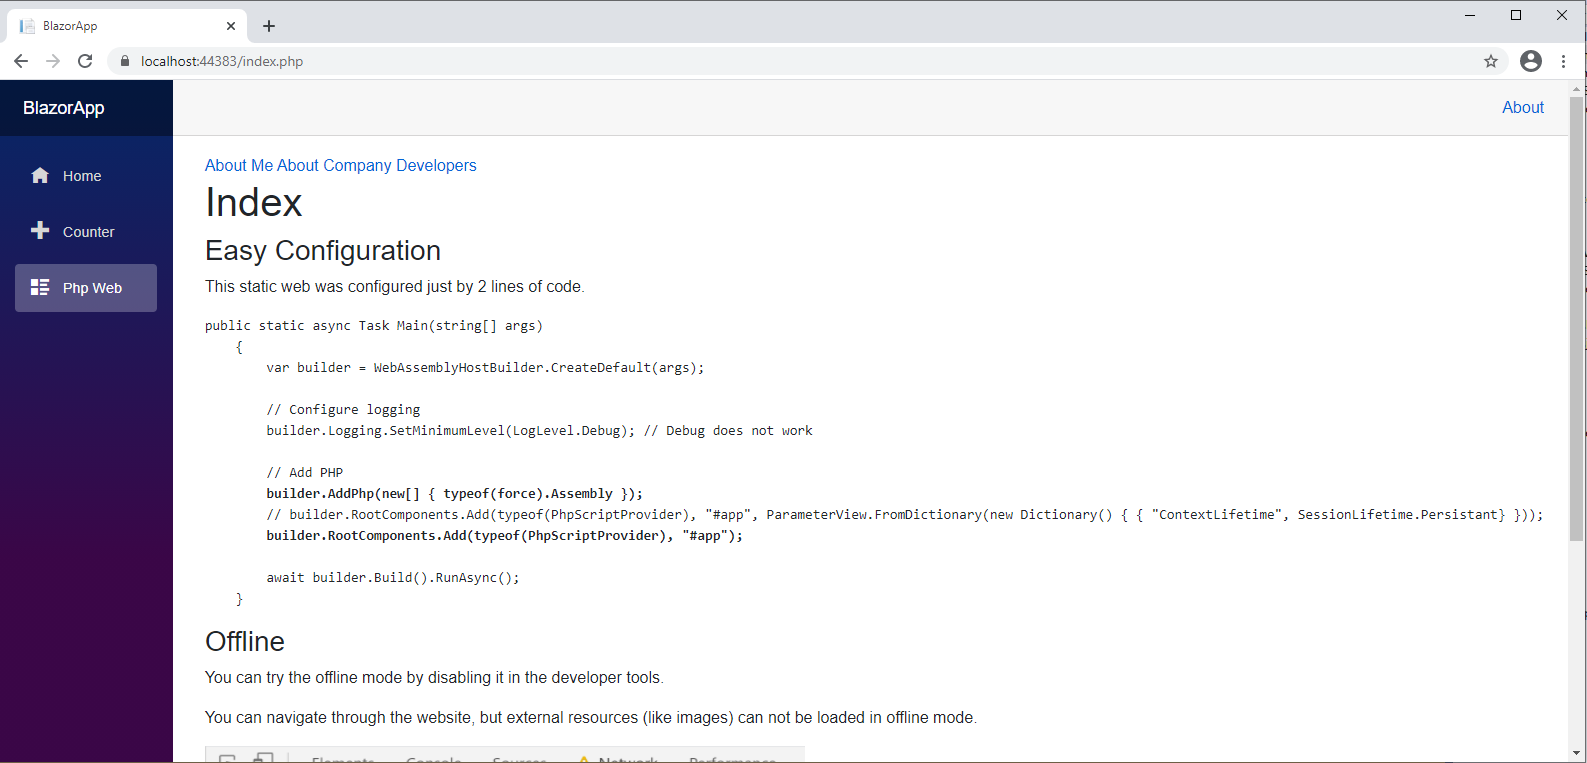
\includegraphics[scale=0.4]{./img/AllTogether}
\caption{The example.}
\label{img30:allTogether}
\end{figure} 